\newpage
\section{Intro to self and the workplace}

\subsection{Description}
Tell the reader about you and your work. Include relevant features of yourself, including your learning objectives for this internship, if your background and prior experience had an impact, etc, and include relevant features of your work (role title \& supervisor title, how your unit fits within the organization, location of the internship (e.g. local or international), describe your role and key activities as if to someone unfamiliar with this field, etc).

\subsection{Content}

\subsubsection{About me}
I am currently a third-year Computer Science student at Concordia. 
My focus area in the field is Software Systems. 
With the nature of my study, I am eager to learn about the software development process in depth, from developing to shipping the final product.
Before the internship, mostly I was doing personal projects on my own and sometimes in teams to learn and improve my own skill set.
I also enjoy participating in Hackathons since it is a great chance to meet like-minded people and work on something interesting.

\newpage
\subsubsection{About Theia team at Ericsson}
Ericsson is a multinational networking company and is also a major leader in the domain of telecommunications technology, headquartered in Stockholm.
Theia team fits in the organization as a software team mainly is responsible for maintaining and developing project Eclipse Theia (https://theia-ide.org)
which is a framework to develop Cloud and Desktop IDE (Integrated Development Environment).
Along with the main repository (codebase), the team also works on a variety of support tools.

\begin{itemize}
    \item Main repository: https://github.com/eclipse-theia/theia
    \item https://github.com/theia-ide 
    \item https://github.com/eclipse-theia
\end{itemize}

\begin{figure}[h]
    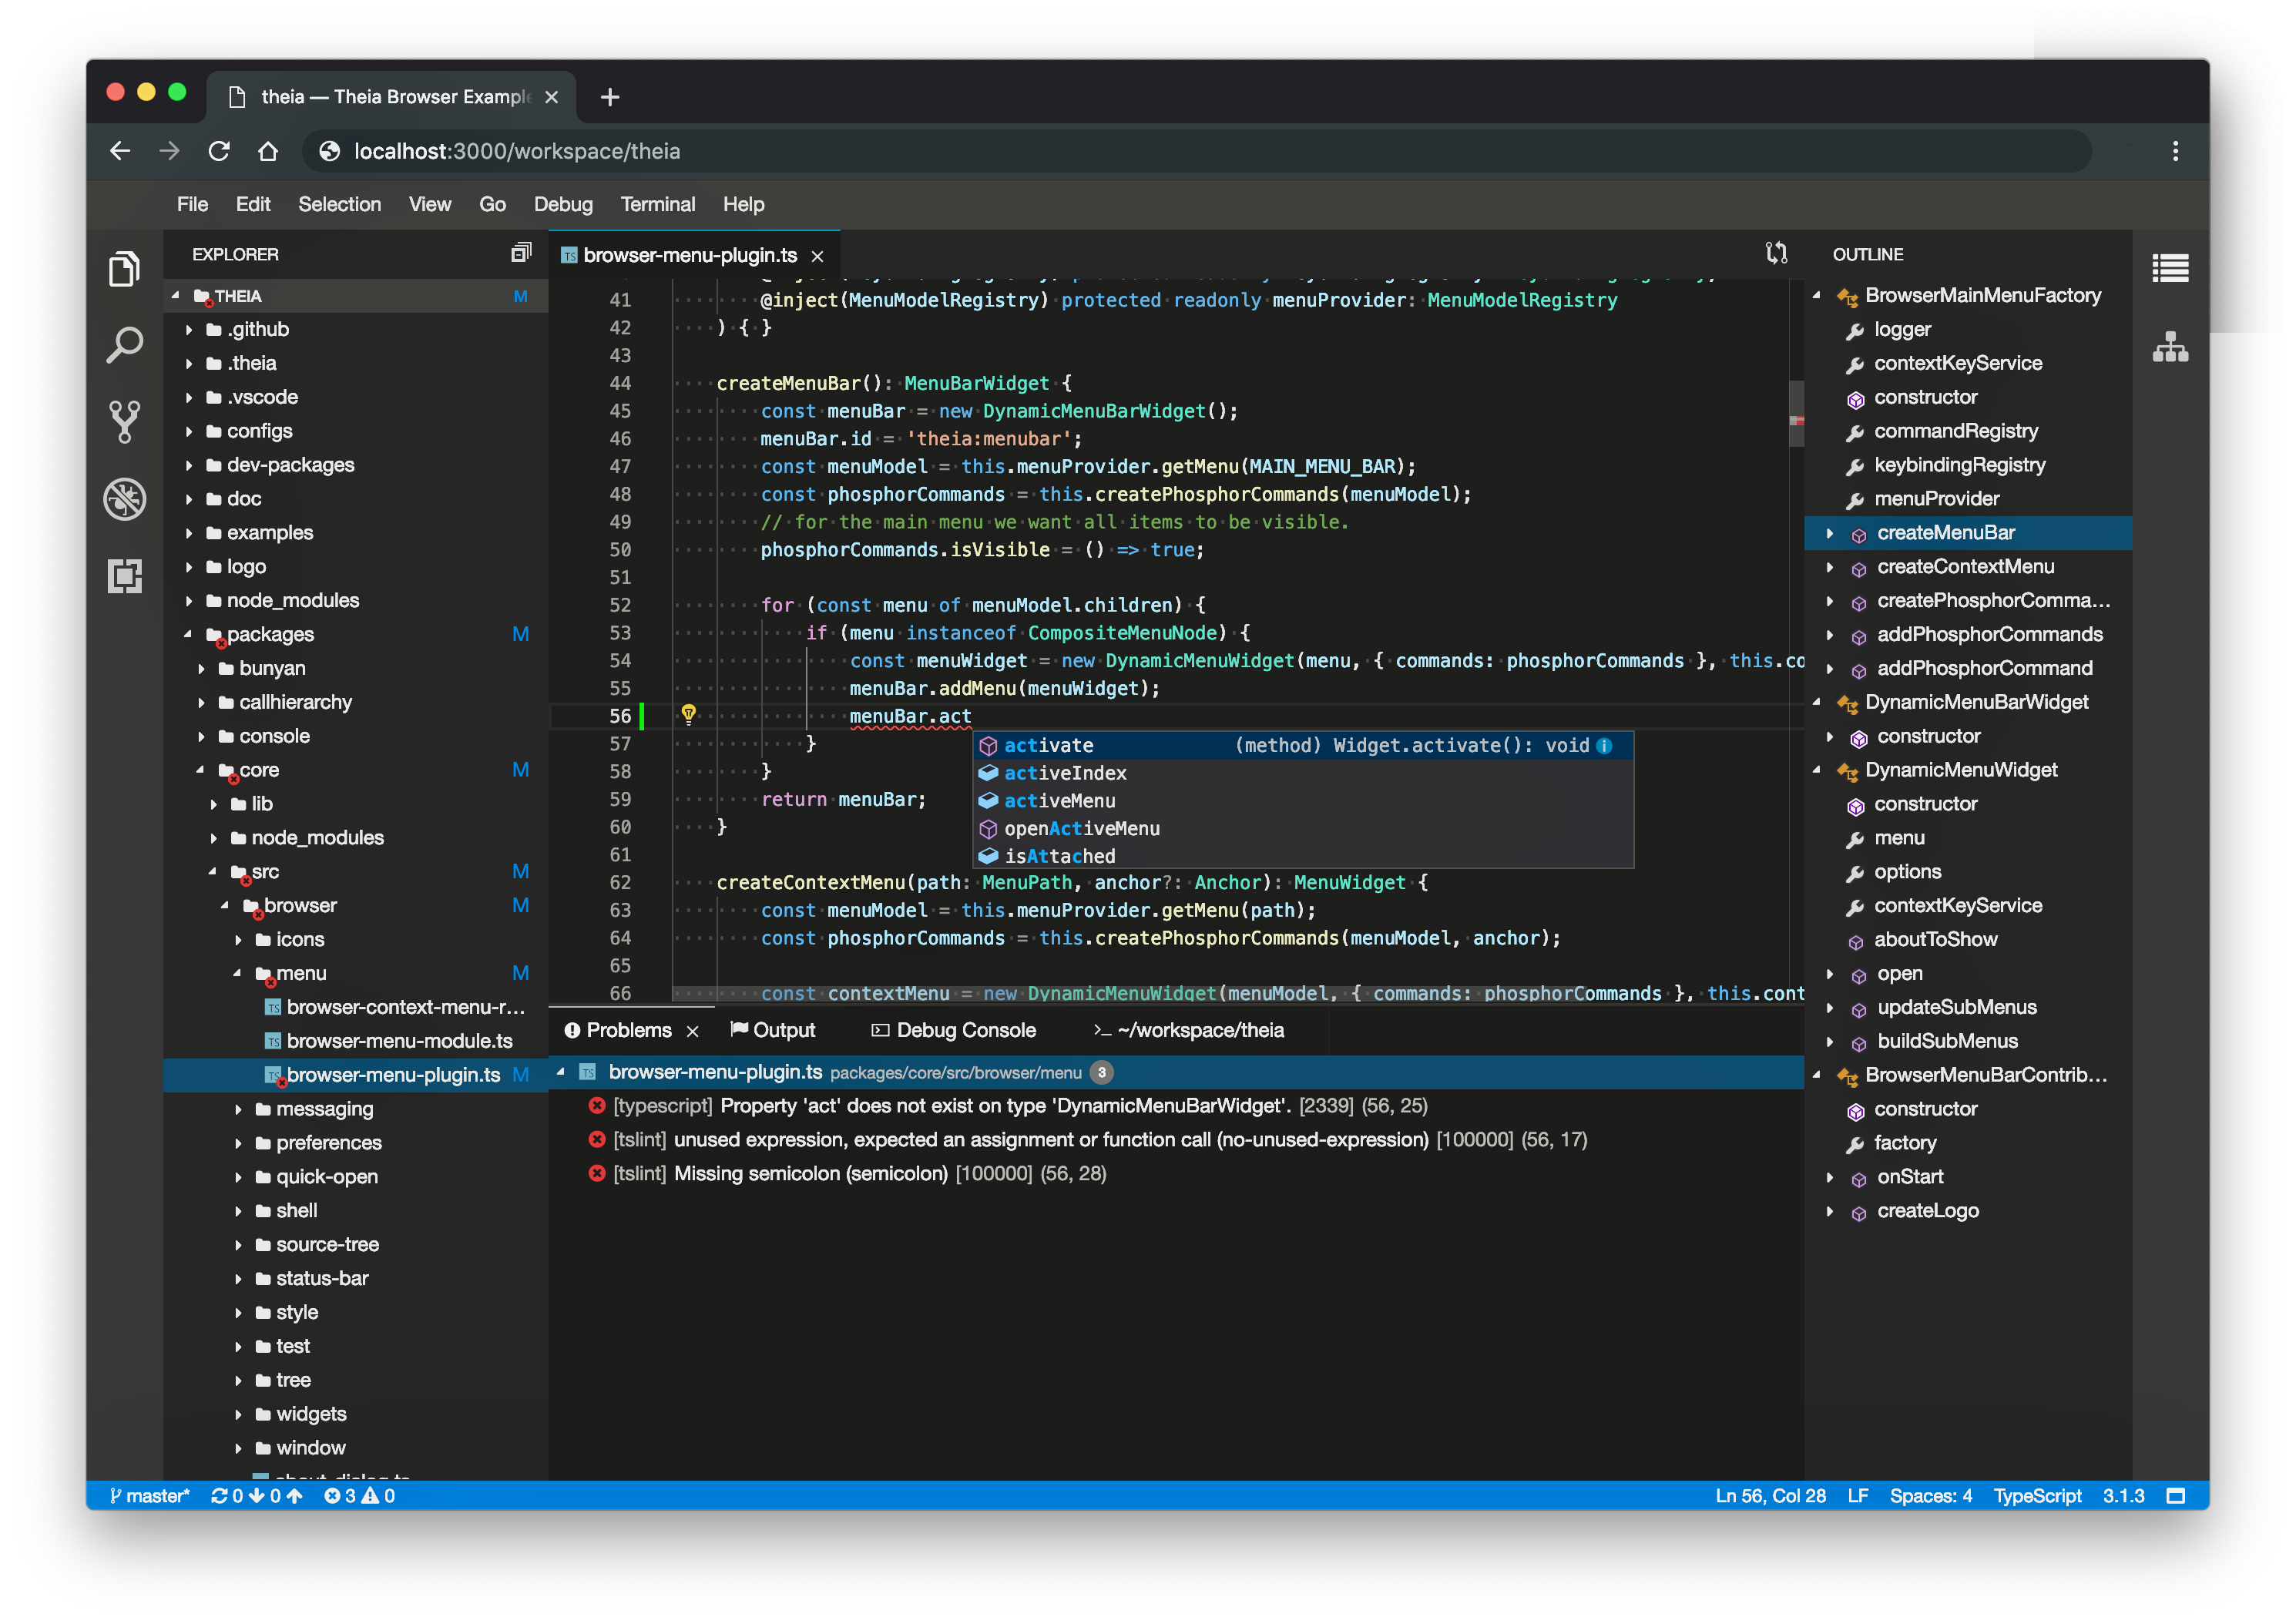
\includegraphics[scale=0.125]{theia}
    \caption{Theia Framework Browser Example}
\centering
\end{figure}

The project is open-source, hence the code base is public and available on GitHub.
With the nature of open-source projects, contribution comes from anyone.
Theia team at Ericsson is only one of the teams contributing to the project, alongside many other companies such as Typefox, SAP, RedHat, Huawei, and more.
\\
\\
With the current COVID-19 pandemic and Canada regulations, all the activities in the internship were done \textbf{remotely (work from home) }

\newpage
\subsubsection{About my role in Theia team}
My role as a Coop Software Developer is to test, investigate bugs, develop, and enhance features in the framework.
Other than that, I also participate in code review for both team members and community contributors.
The team is usually flexible on the tasks I can work with, so I often work on the issues that I find interesting.

